\documentclass[14pt]{extbook}
\usepackage{multicol, enumerate, enumitem, hyperref, color, soul, setspace, parskip, fancyhdr} %General Packages
\usepackage{amssymb, amsthm, amsmath, bbm, latexsym, units, mathtools} %Math Packages
\everymath{\displaystyle} %All math in Display Style
% Packages with additional options
\usepackage[headsep=0.5cm,headheight=12pt, left=1 in,right= 1 in,top= 1 in,bottom= 1 in]{geometry}
\usepackage[usenames,dvipsnames]{xcolor}
\usepackage{dashrule}  % Package to use the command below to create lines between items
\newcommand{\litem}[1]{\item#1\hspace*{-1cm}\rule{\textwidth}{0.4pt}}
\pagestyle{fancy}
\lhead{Progress Quiz 9}
\chead{}
\rhead{Version B}
\lfoot{8590-6105}
\cfoot{}
\rfoot{Fall 2020}
\begin{document}

\begin{enumerate}
\litem{
Determine the appropriate model for the graph of points below.
\begin{center}
    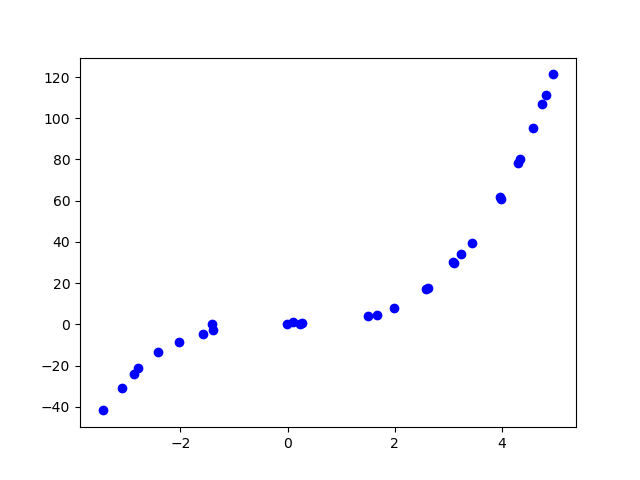
\includegraphics[width=0.5\textwidth]{../Figures/identifyModelGraph12B.png}
\end{center}
\begin{enumerate}[label=\Alph*.]
\item \( \text{Logarithmic model} \)
\item \( \text{Non-linear Power model} \)
\item \( \text{Linear model} \)
\item \( \text{Exponential model} \)
\item \( \text{None of the above} \)

\end{enumerate} }
\litem{
Determine the appropriate model for the graph of points below.
\begin{center}
    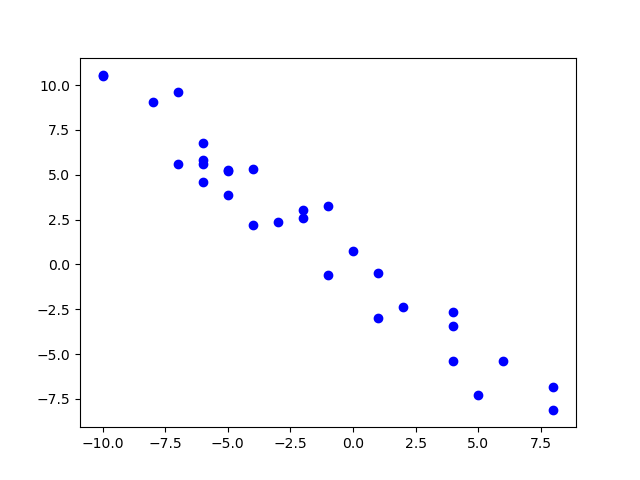
\includegraphics[width=0.5\textwidth]{../Figures/identifyModelGraph12CopyB.png}
\end{center}
\begin{enumerate}[label=\Alph*.]
\item \( \text{Non-linear Power model} \)
\item \( \text{Logarithmic model} \)
\item \( \text{Linear model} \)
\item \( \text{Exponential model} \)
\item \( \text{None of the above} \)

\end{enumerate} }
\litem{
The temperature of an object, $T$, in a different surrounding temperature $T_s$ will behave according to the formula $T(t) = Ae^{kt} + T_s$, where $t$ is minutes, $A$ is a constant, and k is a constant. Use this formula and the situation below to construct a model that describes the uranium's temperature, $T$, based on the amount of time t (in minutes) that have passed. Choose the correct constant $k$ from the options below.
\begin{center}
    \textit{ Uranium is taken out of the reactor with a temperature of $180^{\circ}$ C and is placed into a $19^{\circ}$ C bath to cool. After 16 minutes, the uranium has cooled to $117^{\circ}$ C. }
\end{center}
\begin{enumerate}[label=\Alph*.]
\item \( k = -0.04712 \)
\item \( k = -0.03800 \)
\item \( k = -0.03800 \)
\item \( k = -0.04627 \)
\item \( \text{None of the above} \)

\end{enumerate} }
\litem{
Solve the modeling problem below, if possible.
\begin{center}
    \textit{ A new virus is spreading throughout the world. There were initially 5 many cases reported, but the number of confirmed cases has doubled every 2 days. How long will it be until there are at least 100000 confirmed cases? }
\end{center}
\begin{enumerate}[label=\Alph*.]
\item \( \text{About } 29 \text{ days} \)
\item \( \text{About } 10 \text{ days} \)
\item \( \text{About } 20 \text{ days} \)
\item \( \text{About } 9 \text{ days} \)
\item \( \text{There is not enough information to solve the problem.} \)

\end{enumerate} }
\litem{
Solve the modeling problem below, if possible.
\begin{center}
    \textit{ In CHM2045L, Brittany created a 16 liter 21 percent solution of chemical $\chi$ using two different solution percentages of chemical $\chi$. When she went to write her lab report, she realized she forgot to write the amount of each solution she used! If she remembers she used 16 percent and 30 percent solutions, what was the amount she used of the 16 percent solution? }
\end{center}
\begin{enumerate}[label=\Alph*.]
\item \( 7.12 \)
\item \( 8.00 \)
\item \( 5.71 \)
\item \( 10.29 \)
\item \( \text{There is not enough information to solve the problem.} \)

\end{enumerate} }
\litem{
Solve the modeling problem below, if possible.
\begin{center}
    \textit{ A new virus is spreading throughout the world. There were initially 7 many cases reported, but the number of confirmed cases has doubled every 4 days. How long will it be until there are at least 100000 confirmed cases? }
\end{center}
\begin{enumerate}[label=\Alph*.]
\item \( \text{About } 39 \text{ days} \)
\item \( \text{About } 16 \text{ days} \)
\item \( \text{About } 56 \text{ days} \)
\item \( \text{About } 18 \text{ days} \)
\item \( \text{There is not enough information to solve the problem.} \)

\end{enumerate} }
\litem{
For the scenario below, use the model for the volume of a cylinder as $V = \pi r^2 h$.
\begin{center}
    \textit{ Pringles wants to add 45 \text{percent} more chips to their cylinder cans and minimize the design change of their cans. They've decided that the best way to minimize the design change is to increase the radius and height by the same percentage. What should this increase be? }
\end{center}
\begin{enumerate}[label=\Alph*.]
\item \( \text{About } 13 \text{ percent} \)
\item \( \text{About } 15 \text{ percent} \)
\item \( \text{About } 22 \text{ percent} \)
\item \( \text{About } 20 \text{ percent} \)
\item \( \text{None of the above} \)

\end{enumerate} }
\litem{
For the scenario below, use the model for the volume of a cylinder as $V = \pi r^2 h$.
\begin{center}
    \textit{ Pringles wants to add 43 \text{percent} more chips to their cylinder cans and minimize the design change of their cans. They've decided that the best way to minimize the design change is to increase the radius and height by the same percentage. What should this increase be? }
\end{center}
\begin{enumerate}[label=\Alph*.]
\item \( \text{About } 4 \text{ percent} \)
\item \( \text{About } 13 \text{ percent} \)
\item \( \text{About } 20 \text{ percent} \)
\item \( \text{About } 22 \text{ percent} \)
\item \( \text{None of the above} \)

\end{enumerate} }
\litem{
Using the scenario below, model the situation using an exponential function and a base of $\frac{1}{2}$. Then, solve for the half-life of the element, rounding to the nearest day.
\begin{center}
    \textit{ The half-life of an element is the amount of time it takes for the element to decay to half of its initial starting amount. There is initially 756 grams of element $X$ and after 6 years there is 126 grams remaining. }
\end{center}
\begin{enumerate}[label=\Alph*.]
\item \( \text{About } 730 \text{ days} \)
\item \( \text{About } 2555 \text{ days} \)
\item \( \text{About } 1095 \text{ days} \)
\item \( \text{About } 365 \text{ days} \)
\item \( \text{None of the above} \)

\end{enumerate} }
\litem{
Solve the modeling problem below, if possible.
\begin{center}
    \textit{ In CHM2045L, Brittany created a 25 liter 24 percent solution of chemical $\chi$ using two different solution percentages of chemical $\chi$. When she went to write her lab report, she realized she forgot to write the amount of each solution she used! If she remembers she used 18 percent and 38 percent solutions, what was the amount she used of the 38 percent solution? }
\end{center}
\begin{enumerate}[label=\Alph*.]
\item \( 16.03 \)
\item \( 17.50 \)
\item \( 12.50 \)
\item \( 7.50 \)
\item \( \text{There is not enough information to solve the problem.} \)

\end{enumerate} }
\end{enumerate}

\end{document}